\chapter{s--d-model}
Our model consists of two parts. The first part are the conducting electrons who's Hamiltonian is given by a tight-binding model. These conducting electrons can scatter of impurities in the material leading to having a finite momentum life-time. At the same time the spin of the electrons are coupled to its momentum through spin-orbit interactions, making it possible to transfer this angular momentum to the crystal lattice. The second part is the (anti)ferromagnet which we describe using a Heisenberg model in a classical limit, meaning we replace the spin-operators with vectors that are constrained to lie on a unit-sphere. In order to transfer angular momentum between localized and itinerant electrons, We therefore need to introduce a parameter that couples the spin and magnetic moment locally. Such a parameter is similar to what is found in the s--d model, which couples localized $d$ and itinerant $s$ electrons. 

An attractive model that qualitatively describes magnetization dynamics, driven by electric currents is the s--d model. The model consists of two systems: a lattice with localized magnetic moments and a tight-binding model describing the conducting electrons. A phenomenological parameter denoted $\Delta_\text{sd}$, couples the two systems. 

, which allows the transfer of spin angular momentum from one to the other. This simple model is enough to describe a whole range of phenomena, ranging from the Kondo effect to ... 
We are interested in out-of-equilibrium effects in antiferromagnetic materials due to electric current. One attractive option is a honeycomb lattice, such as graphene, as the Fermi-surface close to the $\bb{K}'$ and $\bb{K}$ points are isotropic, making the analysis easy. We can naturally choose the sublattice to have opposing spins, giving rise to antiferromagnetic order. The minimal model that allows us manipulation of the magnetic order by electric current requires two ingredients: spin-orbit interaction for conducting electrons and an s--d-like interaction between conducting and localized electrons. The s--d-like interaction allows transfer of angular momentum between conducting and localized electrons. However, one also requires dissipation of angular momentum, that occurs during scattering of conducting electrons off of impurities. 

In order to derive the result of Eq.~(\ref{diffSOT}) and the expressions for Gilbert damping we shall adopt a particular relaxation model for both spin and orbital angular momenta of conduction electrons. For the model of Eq.~(\ref{TImodel}) those are provided by scattering on disorder potential. We choose the latter 
to be the white-noise Gaussian disorder potential that is fully characterized by a single dimensionless parameter $\alpha\ll 1$,
\be
\label{disorder}
\la V(\bb{r})\ra =0,\quad \la V(\bb{r}) V(\bb{r}') \ra = 2\pi \alpha\, (\hslash v)^2\,\delta(\bb{r}-\bb{r}'),
\e
where angular brackets stay for the averaging over the ensemble of disordered systems. 

The main building block of our analysis is the averaged Green's function in the first Born approximation
\be
\label{green}
G^{\mathrm{R}}_{\bb{p},\ep} = \frac{\ep^\textrm{R} + v(\bb{p}\times \bb{\sigma})_z-\Delta^{\textrm{R}}_z\sigma_z}
{(\ep^{\textrm{R}})^2-v^2p^2 -(\Delta^{\textrm{R}}_z)^2},
\e
where the complex parameters $\ep^\textrm{R}=\ep(1+i\pi \alpha/2)$ and  $\Delta^\textrm{R}_z= \Delta_z(1-i\pi \alpha/2)$ are found from the corresponding self-energy 
\be
\label{Sigma}
\Sigma^{\mathrm{R}}(\ep)  = 2\pi \alpha\,v^2\!\! \int\!\frac{d^2\bb{p}}{(2\pi)^2}G^\mathrm{R}_{\bb{p},\ep}, 
\e
that gives rise to  $\im \Sigma^{\mathrm{R}}= - \pi \alpha (\ep -\Delta_z \sigma_z)/2$  (strictly speaking, the RG analysis \cite{ivan} has to be applied). In the Green's function of Eq.~(\ref{green}) we shift the momentum $\bb{p}$ such that there is no direct dependence on the in-plane magnetization components $m_x$ and $m_y$. 

The next step in disorder-averaging requires the computation of vertex corrections. This means we need to replace the spin operator $\sigma_\alpha$ with a vertex corrected spin operator $\sigma_\alpha^\text{vc}$ in the ladder approximation as depicted in Fig.~\ref{fig:diagrams}(e). The crossed diagrams in Fig.~\ref{fig:diagrams}(b-d) give a contribution to the components of $\hat{K}$ of the order $\mathcal{O}(\alpha^0)$. The
only components that are modified to this order are those
corresponding to the Hall conductivity (i.e. $\sigma_{xy}$ and $\sigma_{yx}$). Details of this calculation can be found Ref.~\cite{ivan}.
%

The dressing of $\sigma_\alpha$ with a single disorder line is denoted by $\sigma_\alpha^{1\times\text{dr}}$ and is conveniently represented in the matrix form by introducing a matrix $\hat{M}$ with $16$ components $M_{\alpha\beta}$ for $\alpha,\beta=0,x,y,z$ (with $\sigma_0=1$)
    \begin{align}
       \sigma_\alpha^{1\times\text{dr}}  = 2\pi \alpha\, v^2 \int\!\frac{d^2\bb{p}}{(2\pi)^2} G^\text{A}_{\ep+\omega,\bb{p}+\bb{q}}\sigma_\alpha G^\text{R}_{\bb{p}} = \pi\alpha M_{\alpha\beta}\sigma_\beta,
        \label{chap1:eq:myseries}
    \end{align}
where the summation of the repeating index $\beta=0,x,y,z$ is assumed. Full expressions of the components of $\hat{M}$ up to second order in $\omega$ and $q$ are given by Eq.~(\ref{chap1:eq:M}a-f). 
%%%
% Fig. 2
%%%
\begin{figure}[t]
\centering
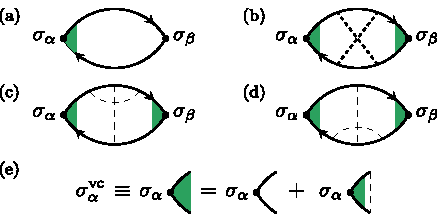
\includegraphics[]{articles/dirac_fm/fig2}
\caption{Diagrams considered in the calculation of $\hat{K}$: (a) non-crossing diagram, (b) $X$ diagram, (c-d) $\Psi$ diagrams. Green areas indicate the ladder summation (e) for the vertex correction in the non-crossing approximation \protect\cite{ivan}.}
\label{fig:diagrams}
\end{figure}

In our calculation the terms of the order of $\alpha \ln p_\textrm{cutoff}/\ep$ (where $p_\textrm{cutoff}$ is the ultraviolet momentum cut-off) is disregarded with respect to $1$. This approximation is legitimate since we assume that all model parameters $\epsilon$, $\Delta_\textrm{sd}$ and $\alpha$ are first renormalized such that $p_\textrm{cutoff} \approx \ep$.

It is, then, easy to see that the vertex-corrected spin operator is readily obtained from the geometric series of powers of $\pi\alpha \hat{M}$, 
\begin{align}
\sigma_\alpha^\text{vc} &= 
\sigma_\alpha+\pi\alpha \hat{M}_{\alpha\beta}\sigma_\beta+(\pi\alpha)^2 (\hat{M}^2)_{\alpha\beta}\sigma_\beta+\dots\nonumber\\
&=\left[1-\pi\alpha \hat{M}\right]^{-1}_{\alpha\beta}\sigma_\beta.
\end{align}
Thus, in the non-crossing approximation (illustrated in Fig.~\ref{fig:diagrams} (a)), one simply finds $\hat{K}= \hat{M}[1-\pi\alpha \hat{M}]^{-1}$. 